\section{Index data and stylized facts of financial returns}
\label{section: Data}

\textbf{Generelt skal den her sektion genovervejes kraftigt - 1. om den overhovedet skal med og 2. hvis den skal, så skal den cuttes kraftigt ned i sideantal og cleanes meget op - bl.a. ala nogle af de kommentarer der er sat med fed ved nogle af outputsne. Derudover, hvis den skal med skal den enten modiferes så den passer bedre ind der hvor den er nu eller flyttes længere ned i opgaven.}

In this chapter, the data used to uncover the economic regimes are introduced. The primary index that will be used to estimate the parameters of the HMM is the S\&P 500 as this is one of the most renowned and liquid stock indices containing some of the largest blue chip companies in the US, and its data dates back long enough to be sufficient for training unsupervised machine learning models. Initially, the choices and associated consequences related to time horizon and optimal observation frequencies are discussed. Secondly, once the data of the S\&P 500 index has been introduced and reviewed its distributional and temporal properties are explored in section \ref{subsection: distributional properties} and \ref{subsection: temporal properties}. The objective of the chapter is thus to provide an overview of the data that serves as potential usage for regime detection along with its statistical properties. The reader should note that an extensive analysis of the stylized facts associated with the empirical data as well as the estimated models will be conducted in section \ref{Section: Stylized facts}.  

\subsection*{Time horizon and frequency of data}
\label{subsection: Data frequency}
When utilising financial market data to uncover economic regime changes, a natural questions arises in terms of which data frequency to use. As described, the objective of DAA is to rebalance the portfolios once a regime shifts has occurred, hence if the regime detection relies on too infrequent data, there is a high probability that several regime shifts will remain hidden. As such, data frequencies longer than a month is not considered. Furthermore, as previously mentioned, broad macroeconomic data is widely available, however, the data is typically characterised by a data frequency of months or even quarters. Therefore, the data frequency of macroeconomic variables propose a challenge, as historic events has shown that economic regime changes can happen swiftly, evident by the recent COVID-19 recession. As such, monthly data compared to e.g. daily data, greatly increases the risk of slow and insufficient detection of economic regime shifts.
 
Despite of the reasoning just outlined, it should be noted that the use of daily data presents some challenges as well. This is due to the fact that daily returns contain a lot of noise and extreme observations, which are evened out on a monthly basis. Consequently, long-horizon returns tend to be more closely approximated by a Gaussian distribution compared to returns for shorter time horizons (Campbell et al. 1997). As such, short-term data frequencies complicates the modeling significantly, which can lead to sporadic predictions and less persistence in the uncovered economic states. In addition, the use of daily return frequencies makes the aforementioned link to macroeconomic data more difficult to justify, and therefore it becomes challenging, from a macroeconomic perspective, to argue that economic regime shifts occur since there is no tangible macroeconomic evidence to support this before the data gets collected and released. Yet, despite the complications associated with short-term data frequencies, the arguments for considering daily as opposed to monthly data frequencies are compelling. 

Furthermore, despite the aforementioned issues with sporadic predictions due to daily data frequencies, Bulla et al. (2011) argued that by relying on daily data it becomes feasible to apply filters that increase confidence whenever a regime change has been detected. As such, research cements the possible of implementing a waiting scheme, in which the portfolio manager would wait several days, when a regime shifts has been detected, before changing the portfolio allocation, thereby minimizing the risk of re-allocating capital based on a wrong signal. In addition, the use of model predictive control (MPC) in section \ref{Subsection: Model predictive control} makes daily data frequencies more justified, since it is not possible to make better return predictions for the assets than their long-term average. As such, looking only a limited number of days into the future is not just an approximation necessary to make the optimization problem computationally feasible, it is also reasonable due to the nature of financial returns.

Bulla et al. (2011) further argued that the use of daily data frequencies increases the amount of data available for markets characterised by a short lifetime, however, many financial indices are old and for these older indices monthly data is more available than daily data. Unsupervised machine learning models, such as HMMs, require large amounts of data to be trained in order to achieve a desired and comfortable level of predictability and persistence, hence the usage of these heavy data-driven models serves as an argument for relying on monthly data as opposed to daily data. Yet, this thesis favors early detection, due to the reasoning outlined above. As a result, daily data, will be used in the analysis. Additionally, the optimal time horizon used for training the model is debatable, however, it should at least span the time required for a financial cycle to unfold in order to include the performance of DAA strategies in several economic environments. Finally, it should be acknowledged that, the longer the data horizon the more questionable it becomes whether stationarity of the data-generating process can be assumed (Bulla et al. 2011). The following sections will include details on the S\&P 500 index.
 
\subsection{The S\&P 500}
The S\&P 500 is a stock index comprising 500 companies from the U.S. was founded in 1957, however, the index dates back all the way to 1923 where it tracked approximately 90 stocks. The stocks that make up the index are selected by a committee which include representation from all major segments in American industry. As such, contrary to prevailing public sentiment, the index is not simply made up of the 500 largest companies in the U.S. The S\&P 500 is a market-capitalization weighted index in which the 10 largest companies account for 27.5\% of the capitalization as per December 2020. Figure \ref{fig: SP500_index} showcases the development of the S\&P 500 index since origination. 
 
\begin{figure}[H] 
    \centering
    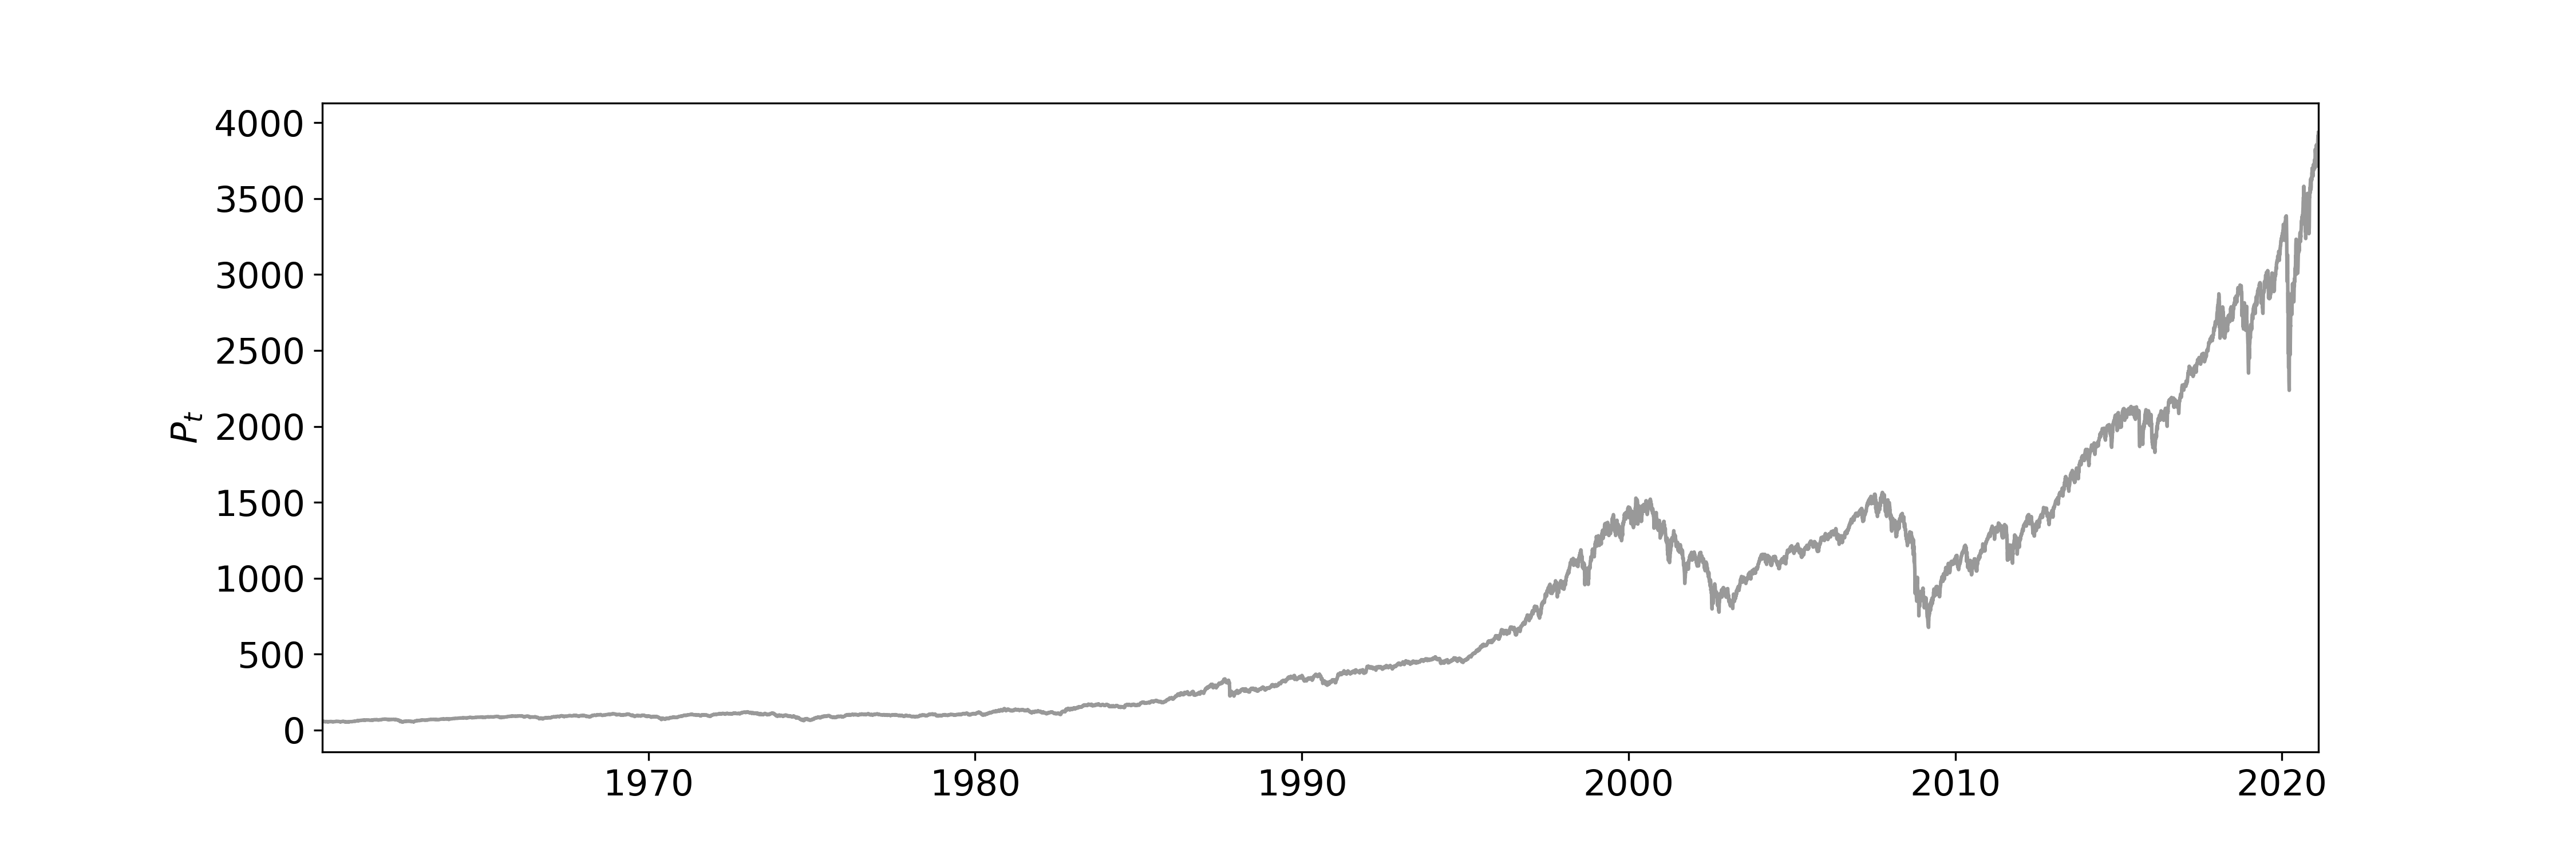
\includegraphics[width=1\textwidth]{analysis/data_description/images/SP500_index.png}
    \caption [Development of the S\&P 500] {Development of the S\&P 500 for the period 01/04/1960 to 12/02/2021.}
    \label{fig: SP500_index}
\end{figure}


As is evident from figure \ref{fig: SP500_index} the 44 years of data has been impacted by the major market movements including Black Monday in October 1987 as well as the dot-com bubble of the late 90s and early 2000s. Furthermore, the attractive bull market leading up to the GFC has been well-captured by the development of the S\&P 500 Index. Lastly, the long bull market following the GFC as well as the recent COVID-19 recession appears to be well-captured by the S\&P 500 Index, thereby indicating that it is adequate for model estimation purposes. In addition, the development following the electronification of financial markets is evident since many actors, including private investors, gained access to the financial markets due to the advancement of technology in the late 90s and early 00s. This is also clearly visible from figure \ref{fig: SP500_index}


From an overall return perspective it is evident that the S\&P 500 index has been subject to a variety of turbulent market periods including the dot-com bubble and most recently the GFC and COVID-19 recession. Interestingly, the S\&P 500 index only recovered from the dot-com bubble a few months prior to the financial crisis of 2008. In the period following the financial crisis the S\&P 500 has been performing increasingly well resulting in an upward trajectory until the recent COVID-19 correction, after which the index reached the present all time high. The fact that the S\&P 500 index has captured the most recent and dramatic market turmoil throughout the last 60 years, further establish that it captures the varying nature of economic regimes. Furthermore, another neat property of the S\&P 500 is the fact that it dates back to 1957, hence there is a large amount of data that can be used to train the subsequent HMMs. For comparison, popular European indices like the DAX 30 originated in 1999, thus shortening the available data considerably.

Additionally, another the choice of relying on the S\&P 500 index for estimation purposes is based on the fact that it is a one of the leading American indices by market capitalization. Secondly, contrary to for instance the Nasdaq Composite Index, the S\&P 500 is not exclusively focusing on a specific sector like information technology, hence it should capture the economics trends across sectors accordingly. As such, the thesis treats it as a baseline index in terms of uncovering economic-regimes. The main critique of using the S\&P 500 index is that it exclusively entails American companies, however, from a macroeconomic perspective the U.S. economy serves as a fundamental leading indicator of how the remaining world economy is progressing, hence it is valid to argue that US stocks will be the first to be impacted by changing economic regime. Taking into consideration the aspect of early regime detection, this means that the fact that the index is composed purely of American companies serves as a strength. Furthermore, North American companies makes up almost 2/3 of alternative indices like the MSCI World, hence no matter which large popular index that will be used, there is bound to be a heavy skew and over-representation towards American stocks.

\subsubsection{Log Returns}
As evident by figure \ref{fig: SP500_index} the series is not stationary since the mean is changing over time, and when zooming in on specific periods, the price development appears to be characterised by strong trends. As such, a transformation is needed to obtain stationary time series. A logarithmic transformation will narrow the gap between the different levels of the index at different periods in time while taking the first difference will eliminate the growing mean values. This results in the log returns being derived as $r_t = log(P_t) - log(P_{t-1})$, where $P_t$ is the adjusted closing price of the index on day $t$ and $\log$ is the natural logarithm. For daily returns less than 10\%, log returns are a good approximation to the discrete return, as it is the first order Taylor approximation (Nystrup, 2014). The plot of the log returns have been shown in figure \ref{fig: log_returns_all_indices}. 

\begin{figure}[H] 
    \centering
    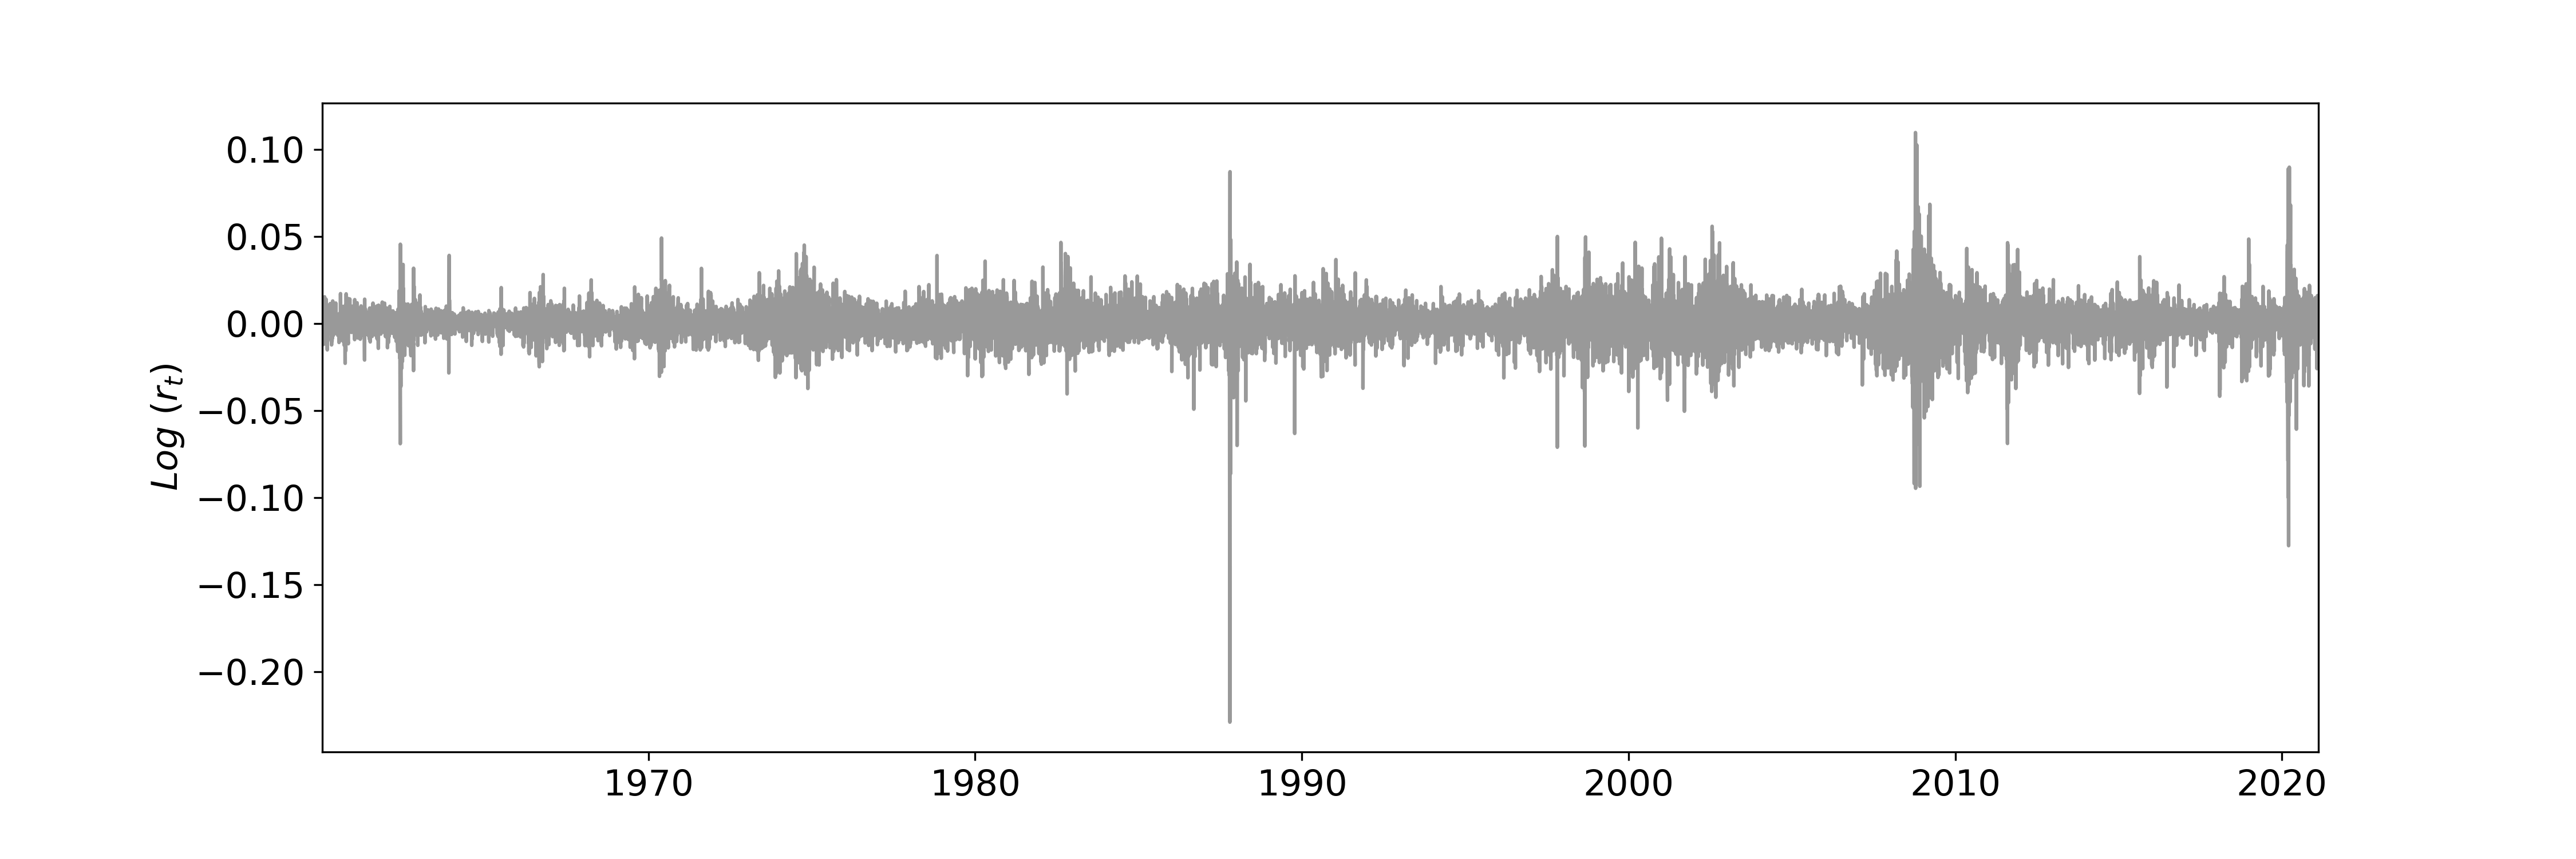
\includegraphics[width=1\textwidth]{analysis/data_description/images/SP500_log_returns.png}
    \caption [Plot of the log returns for the S\&P500 index across time] {Plot of the log returns for the S\&P500 index across time.}
    \label{fig: log_returns_all_indices}
\end{figure}


Evidently, figure \ref{fig: log_returns_all_indices} provides a better overview of the historical market events that have caused extreme observations, for instance the Black Monday event of October 1987 which saw the S\&P 500 index drop by 22.9\% in a single day, hence the observation lies more than 30 standard deviations away from the mean. In order to capture the summary statistics of the daily S\&P 500 log returns, as well as the annual Sharpe ratio and JB statistic, table \ref{tab:summary_stats_S&P500} has been constructed below. As such, it is apparent that the distribution is left skewed and strongly leptokurtic, however, this is not a surprising finding given the studies conducted by Granger \& Ding (1995b) as well as Cont (2001), in which identical stylized facts of financial returns were uncovered and explored substantially. The critical value for the Jarque–Bera test statistic at a 99.9\% significance level is 14.13, hence table \ref{tab:summary_stats_S&P500} clearly highlights that the Jarque–Bera test strongly rejects the hypothesis that the log returns of the S\&P 500 follow a Gaussian distribution.

\begin{table}[H]
\small
\caption{Summary statistics for the daily S\&P 500 log returns.}
\centering
\begin{tabular}{c c c c c c c c c c} 
\hline\hline
Observations\footnote{Time period going from 04/01/1960 to 12/02/2021} & Mean & STD & Skewness & Excess Kurtosis & Min & Max & Annual Sharpe & JB-stat \\
\hline
15,385 & 0.0003 & 0.0103 & -1.0353 & 23.8338 & -0.2290 & 0.1096 & 0.4350 & 27,926 \\
\hline
\end{tabular}
\label{tab:summary_stats_S&P500}
\end{table}
 

\subsection{Distributional properties} 
The recently mentioned left skewness and strong leptokurtotic serve as some of the key distributional properties in regards to the stylized facts of financial returns. In order to graphically illustrate these properties the distribution of the empirical log returns have been plotted in figure \ref{fig: Kernel_distributions} along with a fitted Gaussian and t-distribution. It is clear from the figure that the log return series is characterised by excess kurtosis relative to a Gaussian distribution. As such, there is too much mass centered around the mean and in the tails compared to the Gaussian distribution. In particular, the fat left tail implies that using a Gaussian distribution to model returns will underestimate the frequency and magnitude of downside events (Cont, 2001). 

\textbf{Bør komme som det første i distributional properties. Grafen skal laves om så den baserer sig på standardiserede log returns og farvekoderne skal følges dem fra sektion 5 og fremad.}
\begin{figure}[H] 
    \centering
    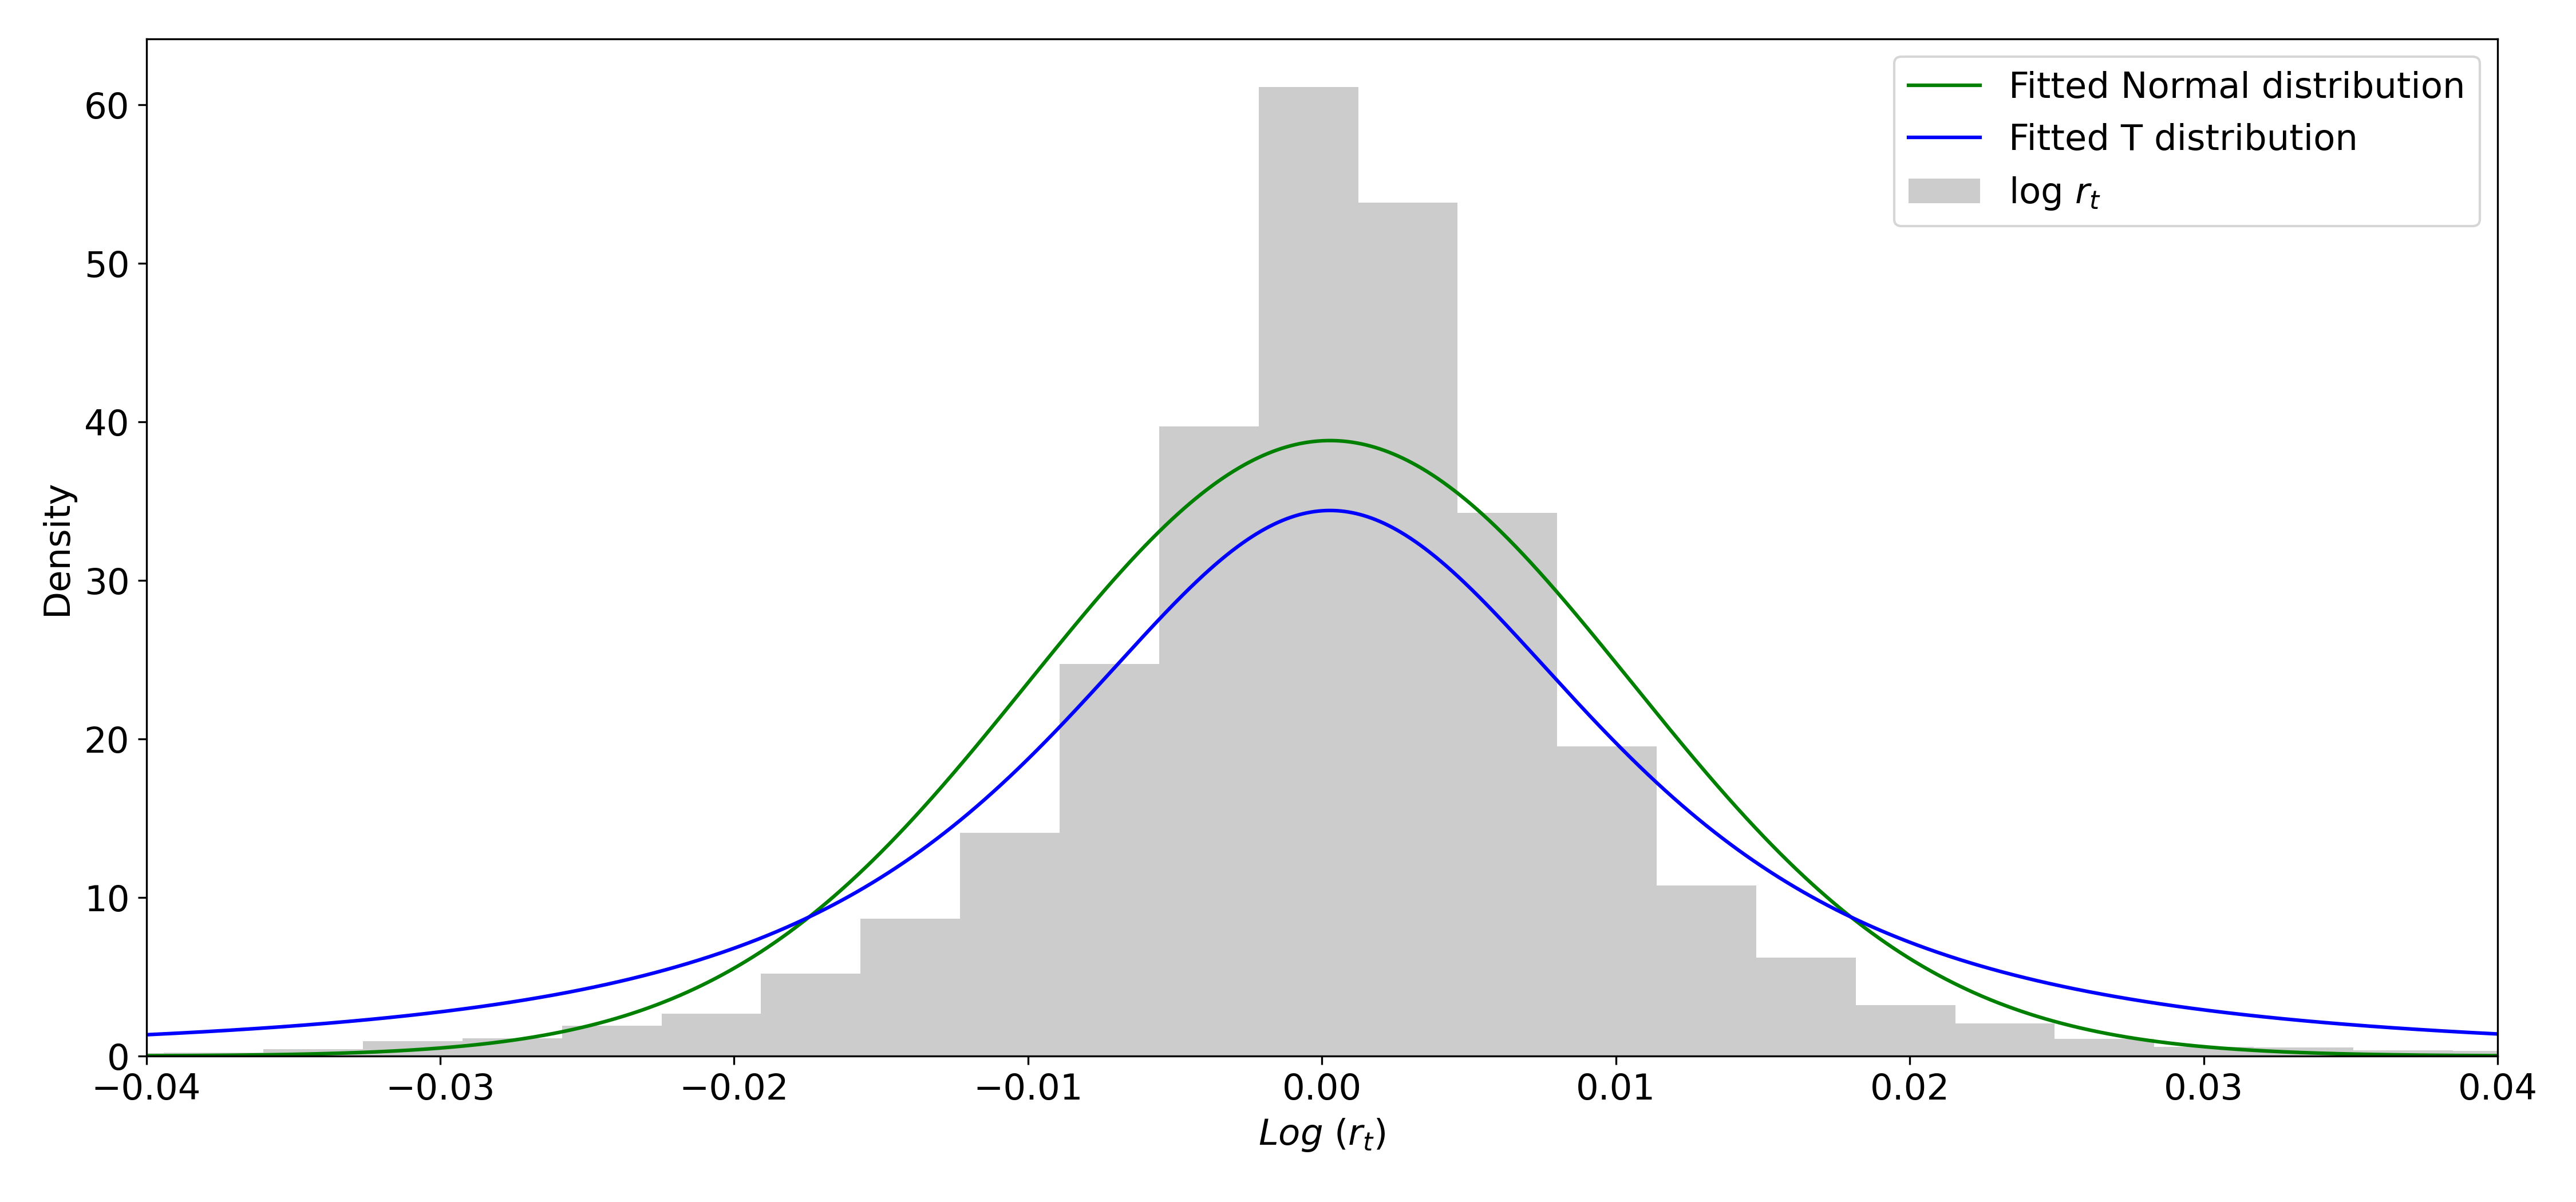
\includegraphics[width=1\textwidth]{analysis/data_description/images/SP500_distribution.png}
    \caption[Density plot of the S\&P 500 log returns] {Density plot of the S\&P 500 log returns. The gray bars highlights the empirical distribution, the green curve is the fitted Gaussian distribution and the blue curve is the fitted T-distribution with XXX degrees of freedom.}
    \label{fig: Kernel_distributions}
\end{figure}

Following the properties that are evident from figure \ref{fig: Kernel_distributions}, an interesting analysis would be to uncover how many observations that lie more than 3 standard deviations from the mean. In total there are 219 observations that lie more than 3 standard deviations away from the mean which is way above the expected 46 if the series followed a Gaussian distribution. Out of these, 108 observations are located in the right side of the tail while the remaining 111 are located in the left tail. This phenomenon that large drawdowns occur more often than similar large upwards movements is well researched and known as the gain/loss asymmetry (Cont, 2001). In addition, it should be noted that since the S\&P 500 index contains 15,385 observations, it only takes a few outliers to reject that the series follows a Gaussian distribution. However, as noted by Cont (2001), financial returns are characterised by a large degree of extreme observations compared to the Gaussian distribution, which is also evident by the large excess kurtosis from table \ref{tab:summary_stats_S&P500}, hence the results are in line with expectations.

Lastly, it is important to note the subtle distinction between outliers and extreme observations since extreme observations deviate considerably beyond 3 standard deviation from the mean, yet they may still hold meaningful information hence they should not be disregarded without further analysis.
Since extreme events happen in live markets the observation that they create should, in some cases, be included in the model estimation in order for the model be as realistic as possible. The other side of the argument is that depending on the extremeness of the observations, they could potentially have severe impact on parameter estimation for the model, thereby serving as an argument for disregarding the extreme observations (Nystrup, 2014). 


\label{subsection: distributional properties}

\subsection{Temporal properties}
\label{subsection: temporal properties}
It is evident by the plot in figure \ref{fig: log_returns_all_indices} that the log returns are characterised as mean stationary, since they fluctuate around a constant level close to zero. Despite this, the log returns series is seen to be more volatile in some periods, for instance during Black Monday in 1987. The effect that large price movements tend to be followed by other large price movements, but not necessarily in the same direction, is known as volatility clustering and it is one of the stylized facts that is hardest for mathematical models to reproduce (Cont, 2001). However, it has been proven that regime-switching models replicate the absence of linear autocorrelation and the long-term memory property of the absolute autocorrelation function well, although simple regime-switching models struggle to achieve a simultaneous fit of the
different stylized facts (Rogers \& Zhang, 2011). Further analysis of this will be conducted in section \ref{Section: Stylized facts}, in which the thesis aims at achieving a simultaneous fit of the stylized facts defined by Granger \& Ding (1995b) through different estimation procedures of the HMMs.

It is particularly evident from figure \ref{fig: log_returns_all_indices} that the S\&P 500 index appears to have increasing volatility through time. This is not a surprising finding since the S\&P 500 index includes observations from the 1960s. During these early days of the financial market, there were no active derivative markets and much fewer actors had direct access to trading financial instruments. As such, markets were simpler, less risky and thus characterised by an overall lower level of volatility compared to the past 40 years of development.

\begin{figure}[H] 
    \centering
    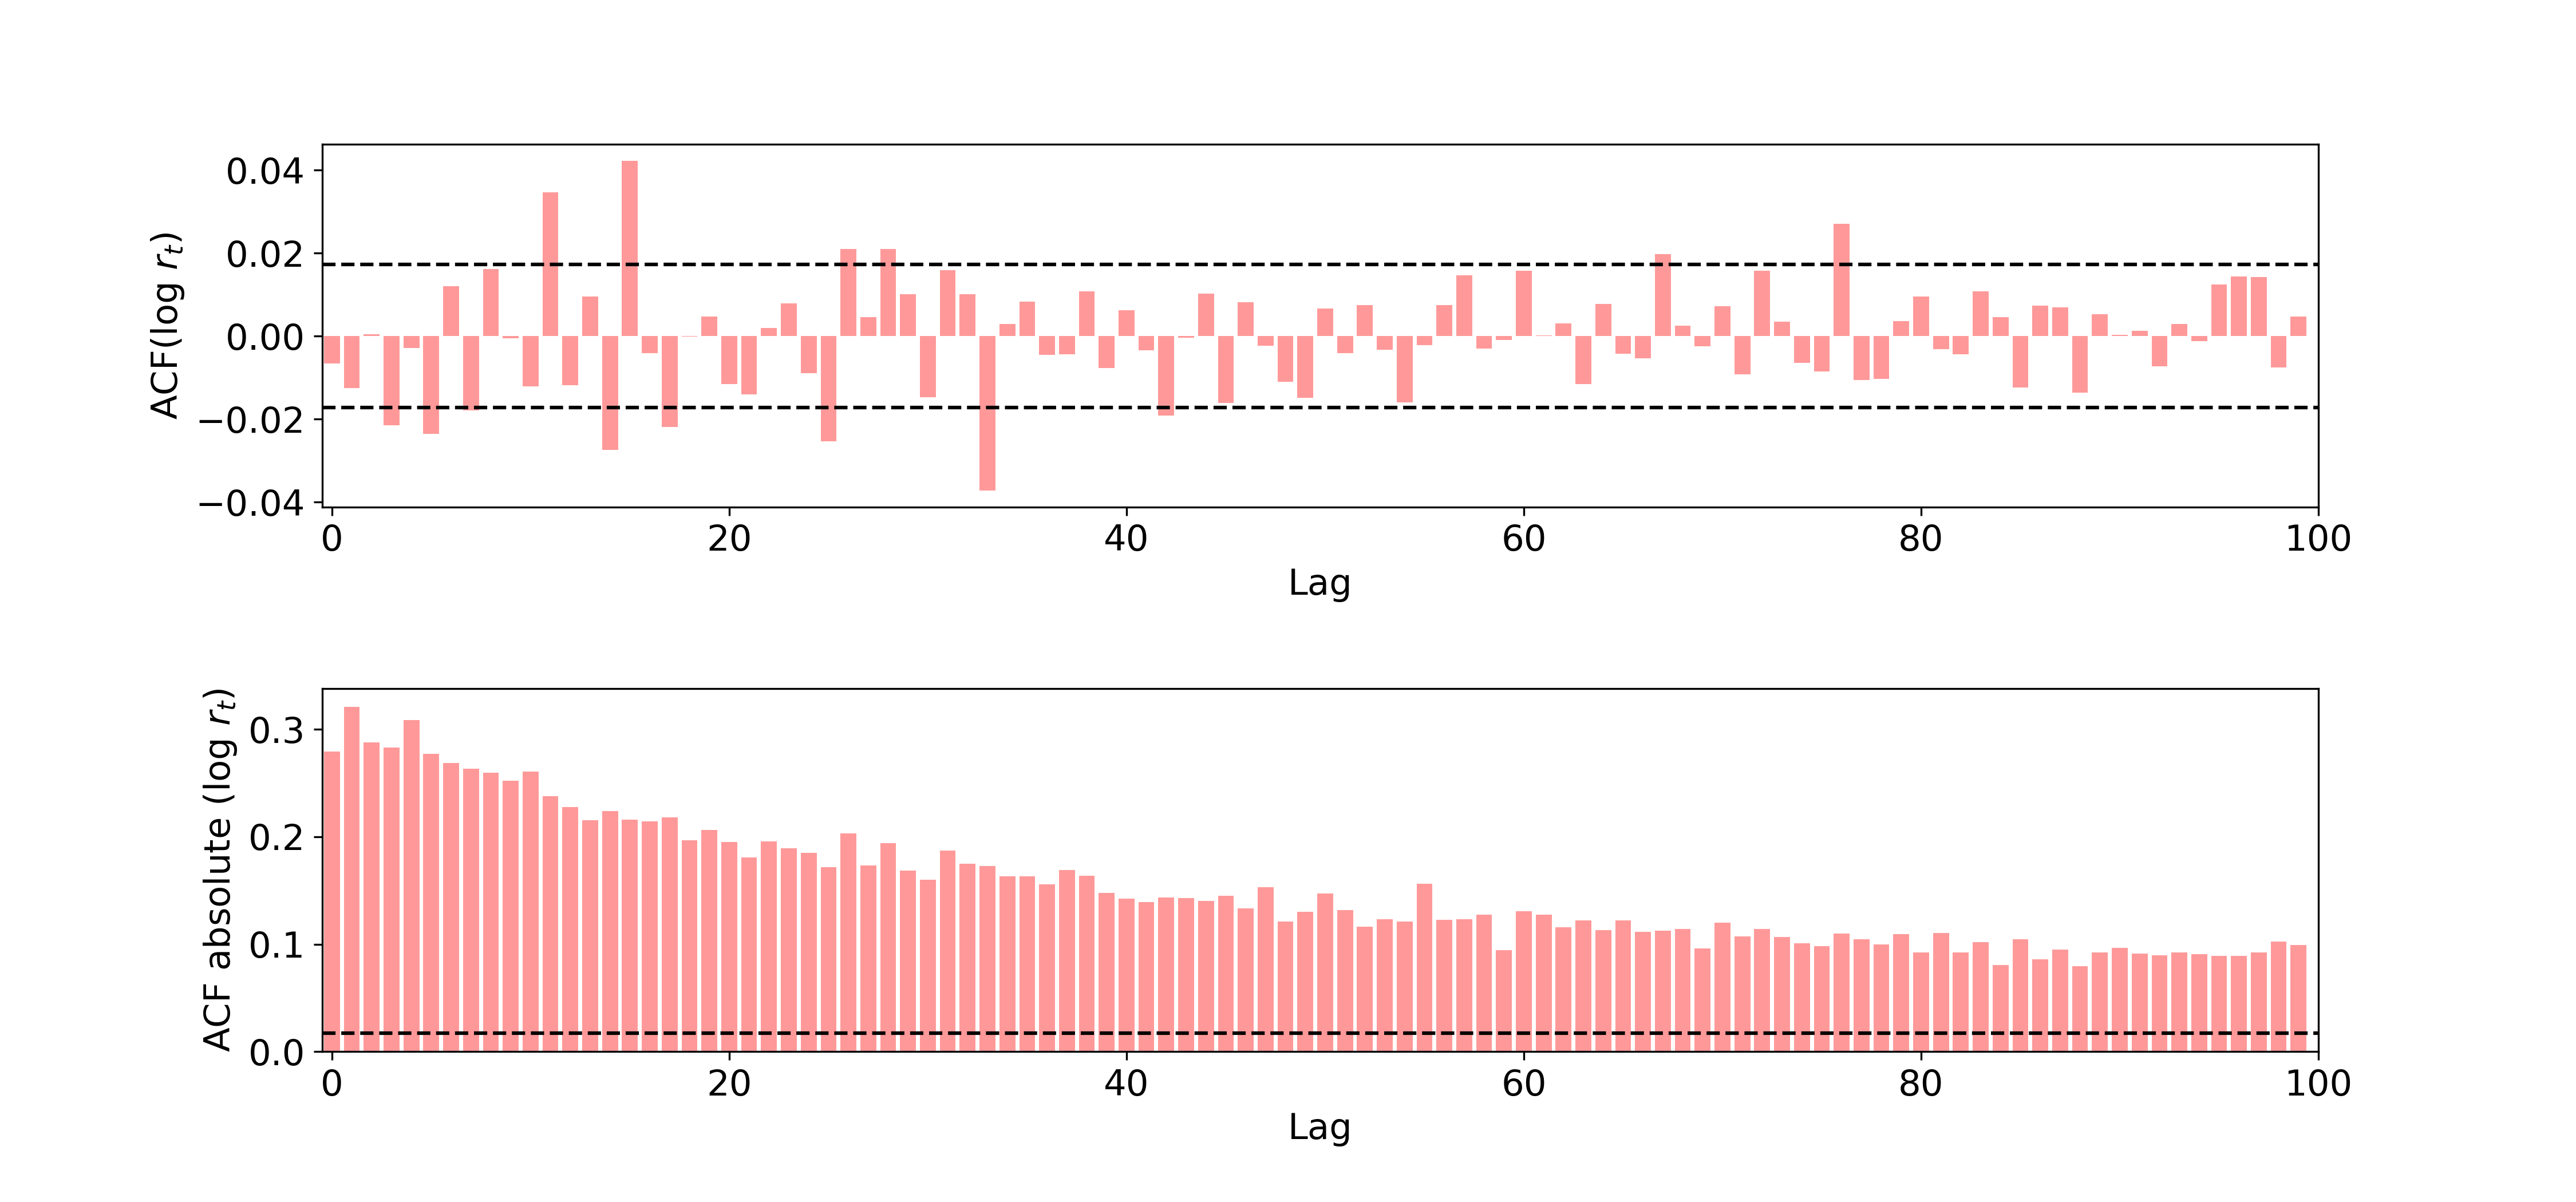
\includegraphics[width=1\textwidth]{analysis/data_description/images/SP500_ACF.png}
    \caption[ACF and absolute ACF for the S\&P500]{ACF and absolute ACF for the S\&P500. The dashed black lines represent the 95\% significance level.}
    \label{fig: ACF_all_log_returns}
\end{figure}

The autocorrelation function (ACF) for the log returns and the absolute log returns are shown in figure \ref{fig: ACF_all_log_returns}. As such, it is evident that the vast majority of the first order linear autocorrelation, at different lags, appears to be non-significant which is in accordance with the empirical studies conducted by Granger \& Ding (1995b) as well as Cont (2001). The fact that some of the lags are significant comes at no surprise either since, as previously discussed, large historical market events such as Black Monday could trigger significant linear autocorrelation, however, this is clearly not persistent across time. Contrary, the absolute ACF of the log returns is significant all the way up to lag 100. This suggests that financial returns exhibit a memory component, thereby making volatility somewhat predictable. As such, the long memory of the absolute log returns is closely related to the previously described volatility clustering from figure \ref{fig: log_returns_all_indices}. This finding is also congruent to the aforementioned empirical studies. The following section will briefly introduce the notation as well as some of the prominent literature associated with HMMs.
